\documentclass[runningheads]{llncs}

\usepackage[T1]{fontenc}
\usepackage[utf8]{inputenc}
\usepackage{graphicx}
\usepackage{booktabs}
\usepackage{amsmath}
\usepackage{amssymb}
\usepackage{siunitx}
\usepackage{xcolor}
\usepackage{microtype}
\usepackage[hidelinks]{hyperref}
\usepackage{xspace}

\graphicspath{{figures/}}

% compact tables
\setlength{\tabcolsep}{4.5pt}
\renewcommand{\arraystretch}{1.05}
\setlength{\textfloatsep}{8pt plus 2pt minus 2pt}
\setlength{\intextsep}{8pt plus 2pt minus 2pt}
\setlength{\abovecaptionskip}{4pt}
\setlength{\belowcaptionskip}{2pt}

% --- convenience macros -------------------------------------------------------
\newcommand{\ie}{i.e.\xspace}
\newcommand{\eg}{e.g.\xspace}
\newcommand{\bridge}[1]{\texttt{#1}}
\newcommand{\ntiles}{\ensuremath{n_{\text{tiles}}}\xspace}
\newcommand{\multitoken}{\bridge{multi\_token}\xspace}
\newcommand{\dF}{\ensuremath{\Delta}F1\xspace}
\newcommand{\dCiderD}{\ensuremath{\Delta}CIDEr-D\xspace}
% CIDEr-D etc. reported x100 throughout.

\begin{document}

\title{Improving a Frozen-Backbone Vietnamese VLM Cheaply:\\
A Six-Question Diagnosis of the Bottleneck}
\titlerunning{Improving a Frozen-Backbone Vietnamese VLM Cheaply}

\author{Anonymous}
\authorrunning{Anonymous}
\institute{Anonymous}

\maketitle

\begin{abstract}
Adapting a strong Vietnamese vision--language model such as Vintern-1B to a new
benchmark is expensive: its own recipe fully fine-tunes the vision encoder and
projector and LoRA-tunes the decoder over millions of pairs, and a recent
alternative, ViMoE-VQA, discards the backbone and trains a new mixture-of-experts
model from scratch. We ask whether the existing model can instead be improved
\emph{cheaply} --- both backbones frozen, ${\sim}1\%$ of parameters trainable, a
single image tile --- and, where that falls short, \emph{where the bottleneck
is}. A frozen-backbone multi-token bridge at one tile already beats the fully
fine-tuned Vintern-1B on BLEU, METEOR and CIDEr; a rank-16 LoRA on the decoder's
attention projections (a further $0.23\%$ of parameters) lifts token-F1 from
$49.6$ to $54.7$ and puts the recipe above Vintern-1B on every generation metric,
holding up on a held-out test split. We then run a six-question ablation ladder
over the vision and language sides of the frozen model. Five vision- and
training-side levers --- a $10\times$-larger bridge, more image tiles, a learned
per-question routing policy, multi-reference training, and projector-level
representation alignment --- leave token-F1 unchanged or worse (alignment is an
absolute null, \dF{}~$-0.03$). The one lever that helps is the decoder-attention
LoRA, and it helps on every bridge architecture, with a larger effect on weaker
bridges, after which all five bridges collapse into a $0.6$-point F1 band. Moving
the same budget to the decoder's feed-forward layers diverges training. The
useful headroom is specifically in the frozen decoder's attention, not the visual
pipeline. This is also a direct counterpoint to ViMoE-VQA's ``reasoning-aware''
account: on the same benchmark, question type carries no usable signal about how
much visual computation a question needs.

\keywords{Vietnamese VQA \and frozen-backbone VLM \and parameter-efficient
adaptation \and LoRA \and ablation}
\end{abstract}

\section{Introduction}
\label{sec:intro}

Vietnamese visual question answering (VQA) has a small number of strong open
models. \textbf{Vintern-1B}~\cite{vintern1b} is representative: a
1-billion-parameter vision--language model (VLM) that pairs an
InternViT-300M~\cite{internvl} encoder with a Qwen2-0.5B~\cite{qwen2} decoder
through a two-layer MLP projector, and reaches state-of-the-art accuracy on
Vietnamese VQA benchmarks. Its strength comes at a cost, however. Adapting
Vintern-1B to a new benchmark, as its authors do, means fully fine-tuning the
vision encoder and the projector and applying LoRA to the decoder, over roughly
three million image--question pairs. A recent alternative,
\textbf{ViMoE-VQA}~\cite{vimoevqa}, improves accuracy on the
AutoViVQA~\cite{autovivqa} benchmark by discarding this backbone entirely and
training a new mixture-of-experts VLM from scratch. Both routes are expensive,
and both rewrite most of the model.

This paper asks a narrower, more practical question:

\begin{quote}
\emph{Can we improve Vintern-1B on AutoViVQA by training only a small fraction of
its parameters --- freezing the entire backbone --- and if that is not enough,
where exactly is the bottleneck?}
\end{quote}

Concretely, we freeze both the InternViT-300M encoder and the Qwen2-0.5B decoder
and replace the original projector with a small trainable \emph{bridge} module
(0.78\,\% of all parameters). This is the cheapest possible adaptation: no
gradients flow into either backbone, training fits on a single 16\,GB GPU, and
one run takes a few hours rather than days. We then treat the remaining
performance gap as a diagnostic target. There are two places one could spend a
small additional parameter budget --- the \textbf{vision side} (a larger bridge,
more image tiles, adaptive per-question visual compute) or the \textbf{language
side} (a richer training signal, representation alignment to the decoder, or a
light adapter on the decoder itself) --- and we work through six research
questions, one lever at a time, to find which of them actually moves the needle.

\paragraph{Findings.}
\textbf{The recipe works, cheaply.} A frozen-backbone multi-token bridge at one
tile already surpasses the fully fine-tuned Vintern-1B on BLEU ($+9.4$), METEOR
($+5.0$) and CIDEr ($+23.7$), and beats ViMoE-VQA on corpus CIDEr-D, BLEU-4 and
ROUGE-L --- at about 1\,\% of the trainable parameters and no backbone
fine-tuning. A rank-16 LoRA on the decoder's attention projections (a further
$0.23\%$) lifts token-F1 from $49.6$ to $54.7$ and puts the recipe above
Vintern-1B on \emph{every} generation metric. Held-out test numbers match
validation within $0.5$ F1.

\textbf{The bottleneck is the decoder's attention, and nothing on the vision
side.} Of the six interventions, five are on the vision or training side --- a
$10\times$-larger bridge, more image tiles, a learned per-question routing policy,
multi-reference training, and projector-level representation alignment --- and all
five leave token-F1 unchanged or worse (alignment is an absolute null,
\dF{}~$-0.03$). The one that helps is a LoRA adapter on the frozen decoder; it
helps on \emph{every} bridge architecture, with a larger effect on weaker
bridges, after which all five collapse into a $0.9$-point F1 band. Moving the same
budget to the decoder's feed-forward layers instead diverges training. The useful
headroom is specifically in the frozen decoder's attention. This is also a direct
counterpoint to ViMoE-VQA's ``reasoning-aware'' account: on the same benchmark,
question type carries no usable signal about how much visual computation a
question needs.

\paragraph{Contributions.}
\begin{enumerate}
\item \textbf{A parameter-efficient adaptation recipe for Vietnamese VLMs}
  (Sec.~\ref{sec:method}, Sec.~\ref{sec:results}): a frozen InternViT + frozen
  Qwen2 + a lightweight pooled bridge + a rank-16 attention LoRA on the decoder
  --- ${\sim}1\%$ trainable parameters, one 16\,GB GPU, no backbone fine-tuning
  --- that matches or beats a fully fine-tuned Vintern-1B on generation metrics
  and holds up on a held-out test split.
\item \textbf{A systematic bottleneck diagnosis} (Sec.~\ref{sec:ablation}): a
  six-question ablation ladder over the vision and language sides of a
  frozen-backbone VLM. Four independent vision/training-side levers produce no
  lift; only decoder-attention capacity does, on every bridge. We localise the
  ceiling to the frozen decoder's attention projections --- feed-forward LoRA at
  the same budget diverges.
\item \textbf{A reliable evaluation protocol} for AutoViVQA: a leak-free grouped
  70/15/15 split (no image shared across splits), 3-seed means with bootstrap
  confidence intervals, matched validation/test reporting, a human-judgment
  sanity check on the token-F1 metric, and a FLOPs/latency/throughput
  characterisation of the image-tile lever that prior work on this benchmark
  explicitly deferred.
\end{enumerate}

\section{Related Work}
\label{sec:related}

\paragraph{Vietnamese VQA and AutoViVQA.}
Vietnamese VQA has moved from extractive datasets (ViVQA, OpenViVQA, ViTextVQA)
toward free-form generative answering. \textbf{AutoViVQA}~\cite{autovivqa}
provides 19{,}411 images and 37{,}077 questions, each with five free-form answers
and a reasoning-type label, and no public test split; published results span
seq2seq baselines, a fine-tuned \textbf{Vintern-1B}, proprietary LLMs, and
\textbf{ViMoE-VQA}.

\paragraph{Frozen-backbone VLMs and the vision--language bridge.}
A large body of work adapts a frozen image encoder and frozen language model by
training only a small connector --- \textbf{Frozen}~\cite{frozen},
\textbf{BLIP-2}~\cite{blip2} (a Q-Former), \textbf{LLaVA}~\cite{llava} (an MLP
projector, LLM un-frozen). Vintern-1B follows the LLaVA recipe but, downstream,
fully fine-tunes the encoder and projector and LoRA-tunes the decoder; we keep
everything frozen except a lightweight bridge and study a five-design capacity
ladder. ``Inference-Optimal VLMs''~\cite{inferenceoptimalvlms} argues a smaller
LLM with more visual tokens often beats a larger LLM with fewer; our ablations
probe the frozen-backbone version and find the frozen decoder, not the visual
token budget, to be the binding constraint.

\paragraph{Parameter-efficient adaptation, and where in the decoder.}
Parameter-efficient methods insert a few trainable weights ---
\textbf{adapters}~\cite{adapters}, \textbf{prefix / prompt
tuning}~\cite{prefixtuning}, \textbf{LoRA}~\cite{lora}. Two questions the LoRA
literature leaves partly open, and that we address for a frozen-backbone VLM, are
\emph{where} in the decoder the adapter goes and how its benefit interacts with
the connector. Interpretability work casts feed-forward layers as key--value
memories~\cite{ffnkvmemory} and attention as inter-position routing, and
adapter-placement studies find attention-only adaptation often competitive with
adapting all linear layers; our result --- an attention LoRA lifts token-F1 while
a same-rank feed-forward LoRA destabilises training --- is a concrete data point
for frozen 0.5\,B decoders on low-resource generative VQA.

\paragraph{Mixture-of-experts and ``reasoning-aware'' routing.}
\textbf{ViMoE-VQA}~\cite{vimoevqa} improves AutoViVQA accuracy by building a new
generative model (frozen CLIP and PhoBERT, a four-expert Top-2 MoE, a six-layer
decoder, trained from scratch) and attributes part of its gain to
``approximate reasoning-aware expert selection''. We are a direct counterpoint on
the \emph{same benchmark}: we improve the existing Vintern-1B rather than replace
it, and we test the reasoning-aware premise directly
(Sec.~\ref{sec:abl-routing}) --- reasoning type carries no signal about the
optimal visual-compute action, and no learned policy beats a fixed one. ViMoE's
own leave-one-out ablation is consistent (removing any expert moves BLEU by only
$0.11$--$0.44$), suggesting the gain is added capacity rather than specialisation.

\section{Method}
\label{sec:method}

\subsection{Frozen-backbone VLM with a trainable bridge}
\label{sec:method-arch}

Our base model follows Vintern-1B: a vision encoder \textbf{InternViT-300M} and a
language model \textbf{Qwen2-0.5B}, connected by a projector. Unlike Vintern-1B's
own downstream-adaptation recipe (full fine-tuning of the encoder and projector,
LoRA on the decoder), we freeze both backbones and replace only the projector
with a trainable \emph{bridge} module. Training optimises the bridge alone, by
cross-entropy on a reference answer (Fig.~\ref{fig:method}).

\begin{figure}[t]
  \centering
  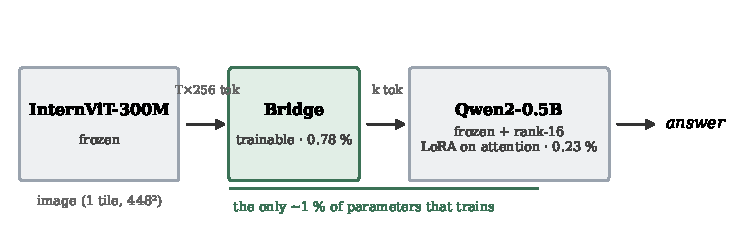
\includegraphics[width=\linewidth]{fig_method}
  \caption{The frozen-backbone architecture. An image is encoded as $1$--$T$
  tiles by a frozen InternViT-300M; a trainable bridge (green, ${\sim}1\%$ of
  parameters) maps the patch tokens to $k$ vision tokens; a frozen Qwen2-0.5B
  decoder --- optionally with a rank-16 attention LoRA --- generates the
  Vietnamese answer.}
  \label{fig:method}
\end{figure}

We study five bridges spanning a capacity ladder from a one-token linear
projector to a 16-query Q-Former (Table~\ref{tab:bridges}). The
\textbf{multi-token bridge} --- eight mean-pooled tokens, one anchor plus seven
semantic --- is our default: it has the lowest trainable-parameter count among
the multi-token designs (0.78\,\%) and the lowest validation cross-entropy of all
five.

\begin{table}[t]
  \centering
  \caption{The five bridge designs, ordered by trainable-parameter count.}
  \label{tab:bridges}
  \begin{tabular}{lccl}
    \toprule
    Bridge & $k$ tokens & Trainable params & Mechanism \\
    \midrule
    Residual        & 1  & 4.86\,M (0.52\,\%) & linear projector $+$ LayerNorm/GELU residual \\
    \textbf{Multi-Token} & 8  & 7.35\,M (0.78\,\%) & mean-pool patches $\rightarrow$ 8 tokens (1 anchor $+$ 7 semantic) \\
    Tile-Attention  & 8  & 4.14\,M (0.44\,\%) & dense patch self-attention, then pool \\
    Light Q-Former  & 8  & 27.6\,M (2.87\,\%) & 8 learned queries, 2-layer cross-attention \\
    Full Q-Former   & 16 & 69.4\,M (6.91\,\%) & 16 learned queries, 4 layers, image--text fusion \\
    \bottomrule
  \end{tabular}
\end{table}

\subsection{Two knobs, one diagnostic ladder}
\label{sec:method-ladder}

Given a frozen backbone, a small additional parameter or compute budget can be
spent on the \textbf{vision side} or the \textbf{language side} of the pipeline.
We work through six research questions, one lever at a time, each measured as
\dF{} against a fixed anchor (the multi-token bridge, one tile, no LoRA):

\begin{table}[t]
  \centering
  \caption{The six research questions. RQ1--RQ4 are vision/training-side; RQ5
  straddles; RQ6 is the language side.}
  \label{tab:rqs}
  \begin{tabular}{clc}
    \toprule
    & Question & Lever \\
    \midrule
    RQ1 & Does a larger / more expressive bridge close the token-F1 gap? & bridge capacity \\
    RQ2 & Is the bridge itself the constraint, or already near-optimal? & validation CE across bridges \\
    RQ3 & Does more visual resolution --- more image tiles --- help? & \ntiles{} \\
    RQ4 & Does \emph{adaptive}, per-question visual-compute allocation help, driven by question type? & router $+$ policy \\
    RQ5 & Does a richer training signal or explicit representation alignment help? & sampling, projector-KD \\
    RQ6 & Does adding capacity to the \emph{frozen decoder} help, and where? & attention vs.\ FFN LoRA \\
    \bottomrule
  \end{tabular}
\end{table}

The shape of the answers --- which levers move F1 and which do not --- is the
paper's main finding (Sec.~\ref{sec:abl-summary}).

\subsection{Adaptive visual computation (RQ3--RQ4)}
\label{sec:method-adaptive}

\paragraph{Tile lever.}
An image is split into $\ntiles \in \{1, 3, 6\}$ tiles of $448{\times}448$; each
tile is a separate InternViT forward pass, so \ntiles{} is the primary
visual-compute knob (Sec.~\ref{sec:abl-compute} characterises its FLOPs/latency
cost).

\paragraph{Router.}
Running in parallel with --- and far more cheaply than --- the vision encoder,
the router produces two signals. A \textbf{cognitive prior} $P(r \mid Q)$: a
PhoBERT head over AutoViVQA's eight reasoning types, seeing the question text only
(validation macro-F1 $0.91$; since the reasoning-type label is largely derivable
from question surface form, this is effectively a question-pattern prior). A
\textbf{cheap visual state} $f(I, Q)$: the InternViT CLS embedding at one tile
(PCA to 64 dims) plus question length and three image scalars (clarity,
occlusion, object density).

\paragraph{Offline oracle-guided policy.}
For a cost trade-off $\lambda$, define the oracle action over the discrete space
$a = (\ntiles, \text{bridge})$ as
$a^\ast(x, \lambda) = \arg\max_a \left[ M(a; x) - \lambda \cdot C(a) \right]$,
where $M(a; x)$ is per-sample CIDEr against the five references and
$C(a) = \ntiles / \max\text{tiles}$. We evaluate \emph{all} actions on
\emph{every} train/val/test question once (the \emph{oracle sweep},
Sec.~\ref{sec:setup-hw}), then train a policy MLP
$\pi_\theta(P(r{\mid}Q), f(I,Q), \lambda)$ by supervised classification against
$a^\ast$ on the training split. Ablation arms differ only in the policy's inputs:
reasoning-type only, visual-state only, both, and fixed / random baselines. RQ4
reduces to whether any learned policy beats the fixed policy ``best bridge at one
tile'' on held-out test.

\subsection{Training-signal and alignment interventions (RQ5)}
\label{sec:method-rq5}

Two ways to give the bridge a better target without touching the backbones:
\textbf{(a) multi-reference answer sampling} --- instead of always training toward
the first of the five references, resample a reference each epoch;
\textbf{(b) projector-level knowledge distillation} --- add a KD term pulling the
bridge output toward Vintern-1B's own pre-aligned \texttt{mlp1} projector, at the
feature level (\texttt{align-feat}) or the decoder-logit level
(\texttt{align-logit}), with weight $\alpha$ on the KD term.

\subsection{Decoder LoRA as a targeted intervention (RQ6)}
\label{sec:method-rq6}

Finally, the smallest departure from ``backbone frozen'': a rank-16 LoRA
($\alpha = 32$, 2.16\,M parameters, $0.23\%$ of the model) on the frozen Qwen2
decoder, trained on top of a fixed bridge. We vary \textbf{which modules} the
LoRA touches --- the attention projections $\{q,k,v,o\}$, the feed-forward
projections $\{\text{gate},\text{up},\text{down}\}$, or all seven --- to localise
where the decoder's useful headroom lies, and vary the number of LoRA epochs
($1$, $3$) to bound the effect.

\section{Experimental Setup}
\label{sec:setup}

\subsection{Dataset and split}

AutoViVQA provides 19{,}411 images / 37{,}077 Vietnamese questions, each with five
diverse free-form answers and a reasoning-type label, released with an 80/20
train/val division and no public test split. We re-partition into a
\textbf{grouped 70/15/15 split}: every image is assigned to exactly one of
train / val / test by hashed \texttt{image\_id} (seed 42), so no image --- and
therefore no shared caption or scene context --- crosses splits, and the
reasoning-type distribution is held approximately fixed across splits.

\begin{table}[t]
  \centering
  \caption{Split statistics. Image overlap between any two splits is $0$.}
  \label{tab:splits}
  \begin{tabular}{lrrrr}
    \toprule
    Split & Questions (eval) & Images & Ans/q & Ans length \\
    \midrule
    Train & ${\sim}25{,}900$ & 13{,}576 & 5.00 & 4.3\,w \\
    Val   & 5{,}463 & 2{,}908 & 5.00 & 4.3\,w \\
    Test  & 5{,}468 & 2{,}914 & 5.00 & 4.3\,w \\
    \bottomrule
  \end{tabular}
\end{table}

A random question-level split gives bridge numbers $\le 0.5$ F1 / $\le 3$ CIDEr-D
higher than this grouped split, so prior AutoViVQA bridge results are not badly
inflated by leakage; we adopt the grouped split for all numbers here.

Reasoning-type (\texttt{category}) distribution: \texttt{relational}
(${\sim}30\%$), \texttt{recognition} (${\sim}19\%$), \texttt{spatial}
(${\sim}15\%$), \texttt{causal} (${\sim}13\%$), \texttt{counting} (${\sim}12\%$),
with \texttt{action}, \texttt{context}, \texttt{yes/no} in the tail. We use the
nominal \texttt{category} labels and treat them as unordered.

The oracle sweep (Sec.~\ref{sec:abl-routing}) evaluates every action on every
question, so it uses an equal-per-category subset
($5{,}547$ / $3{,}727$ / $3{,}739$ questions for train / val / test); overall
means are re-weighted to the natural distribution.

\subsection{Answer selection during training}

Each question has five references. Bridge and LoRA training optimise cross-entropy
against the \textbf{first} reference --- a fixed choice, for reproducibility. All
\textbf{evaluation} uses all five references: per-sample max for token metrics,
corpus multi-reference for CIDEr-D / BLEU / ROUGE / METEOR. Resampling a reference
each epoch (\texttt{answer\_sampling = random}) is one of the RQ5 interventions
(Sec.~\ref{sec:abl-rq5}) and is not otherwise used.

\subsection{Training}

InternViT-300M and Qwen2-0.5B are \textbf{frozen}; only the bridge (and, for RQ6,
a rank-16 decoder LoRA) trains. AdamW, learning rate \num{2e-4}, micro-batch 8, no
early stopping. \textbf{Two epochs} for the bridge: validation cross-entropy
bottoms out within one epoch and corpus CIDEr plateaus by epoch 2 (multi-token
CIDEr $1.025$ at epoch 2 $\rightarrow$ $1.029$ at epoch 4 on an 800-sample
probe), so a third and fourth epoch add nothing and risk instability. The decoder
LoRA is trained for 1 or 3 epochs on top of a fixed bridge
(Sec.~\ref{sec:abl-rq6} reports both). One bridge run is ${\sim}5$ GPU-h; one
LoRA run is ${\sim}3$ (1 epoch) to ${\sim}8$ (3 epochs) GPU-h.

\paragraph{Note on a superseded run.}
One early bridge run trained for four epochs; its seed-42 Residual checkpoint was
a training-instability outlier (validation CE $2.35$ vs.\ $1.5$--$1.7$ for every
other bridge and seed). We re-ran all bridges at two epochs and three seeds; the
sound Residual numbers (F1 $45.6$, CIDEr-D $81.1$) are in line with the other
bridges, and all reported numbers use the two-epoch, three-seed runs. An earlier
auxiliary distillation term (MSE between the bridge's first token and a
linear-projector baseline) is disabled everywhere --- it applied to only two of
the five bridges and is an unfair confound.

\subsection{Hardware, seeds, metrics, statistics}
\label{sec:setup-hw}

All training and evaluation ran on Kaggle P100 (16\,GB) and T4 GPU kernels, no
multi-GPU. Total project compute is on the order of a few hundred GPU-hours; a
single headline recipe run (bridge $+$ 3-epoch LoRA) is ${\sim}13$ GPU-h. Every
bridge and negative-axis intervention and the decoder-LoRA rows are
\textbf{three seeds} ($42$, $123$, $3407$; the multi-token headline row adds
$2026$); oracle / routing runs are seed $42$. We report mean $\pm$ standard
deviation.

Cross-paper generation claims use \textbf{corpus CIDEr-D / BLEU-4 / ROUGE-L}
(pycocoevalcap); METEOR is reported but not used for cross-paper claims (it
varies by ${\sim}13$ points between implementations). Answer matching is
token-level P/R/F1 and exact-match, per-sample max over the five references, from
an in-house scorer whose values match the AutoViVQA baseline table
(Table~\ref{tab:main-inhouse} reports both conventions side by side). Main
comparisons use paired bootstrap ($2{,}000$ resamples); we report $95\%$ CIs on
$\Delta$ quantities and $P(\Delta > 0)$. The full validation split is scored
every run; the \textbf{test split is scored once} and never used for model
selection. Libraries: PyTorch~2, Transformers, \texttt{pyvi}, PhoBERT-base-v2;
InternViT-300M / Qwen2-0.5B from Vintern-1B-v3.5.

\section{Main Results}
\label{sec:results}

Freeze InternViT-300M and Qwen2-0.5B; train only a bridge (the \multitoken{}
projector, 7.35\,M params, $0.78\%$). Optionally add a rank-16 LoRA on the
decoder's attention projections ($q/k/v/o$; 2.16\,M, $0.23\%$), for $1.01\%$
trainable in total. One tile, grouped leak-free 70/15/15 split
(Sec.~\ref{sec:setup}), greedy decoding.

\subsection{Recipe vs.\ prior work}
\label{sec:results-main}

Table~\ref{tab:main-inhouse} reports all AutoViVQA baselines and our recipe on
the eight in-house metrics ($\times 100$). Even the \textbf{bridge alone}
($0.78\%$ trainable, one tile, no LoRA) beats the fully fine-tuned Vintern-1B on
BLEU ($+9.4$), METEOR ($+5.0$) and CIDEr ($+23.7$), and is within ${\sim}4$
points on ROUGE-L. Adding the $0.23\%$ decoder LoRA lifts all four: at
\textbf{3 epochs} the recipe beats Vintern-FT on \emph{every} generation metric
(BLEU $+14.9$, ROUGE-L $+1.0$, METEOR $+10.0$, CIDEr $+36.8$) --- at ${\sim}1\%$
of the trainable parameters, no backbone fine-tuning, and one tile instead of up
to twelve. It also beats ViMoE-VQA on BLEU / ROUGE / METEOR / CIDEr. It trails
ViMoE on token-F1 ($-11.2$ bridge alone, $-7.5$ with 1-epoch LoRA, $-6.0$ at
3 epochs) and Vintern-FT on Acc. Sec.~\ref{sec:ablation} diagnoses where that
remaining F1 gap lives.

\begin{table}[t]
  \centering
  \caption{Recipe vs.\ prior work on AutoViVQA (val), in-house metrics
  ($\times 100$). \textbf{Bold} = ours; baselines as reported by the benchmark.
  BARTPhoBEiT's CIDEr ($188.96$) is a verbosity outlier and omitted.
  $^{\dagger}$ 4-seed (bridge) / 3-seed (+LoRA) mean; std in
  Table~\ref{tab:main-corpus}.}
  \label{tab:main-inhouse}
  \begin{tabular}{lrrrrrr}
    \toprule
    Model & F1 & BLEU & ROUGE & METEOR & CIDEr & Acc \\
    \midrule
    Vintern-1B (base, zero-shot)        & 17.6 & 1.9  & 25.8 & 23.9 & 8.5  & 0.1 \\
    Vintern-1B (fine-tuned, $\le$12 tiles) & 53.8 & 6.1 & 51.9 & 35.3 & 72.8 & 13.0 \\
    GPT-5 (zero-shot)                   & 50.9 & 6.1  & 47.3 & 33.3 & 84.2 & 10.8 \\
    ViMoE-VQA (Tuong-MOE, 5-seed)       & 60.7 & 12.5 & 47.1 & 39.1 & 88.7 & 9.7 \\
    \midrule
    \textbf{Bridge \multitoken{} ($0.78\%$, 1 tile)}$^{\dagger}$ & \textbf{49.55} & \textbf{15.47} & \textbf{47.84} & \textbf{40.22} & \textbf{96.49} & \textbf{8.20} \\
    \textbf{\quad + decoder LoRA r=16 ($1.01\%$)}$^{\dagger}$    & \textbf{53.17} & \textbf{19.44} & \textbf{51.48} & \textbf{43.91} & \textbf{105.59} & \textbf{10.42} \\
    \textbf{\quad + decoder LoRA r=16, 3 epochs}$^{\dagger}$     & \textbf{54.67} & \textbf{20.98} & \textbf{52.92} & \textbf{45.24} & \textbf{109.60} & \textbf{11.78} \\
    \bottomrule
  \end{tabular}
\end{table}

\subsection{Corpus metrics and confidence intervals}
\label{sec:results-corpus}

The in-house metrics match the AutoViVQA convention but are not directly
comparable across implementations. Table~\ref{tab:main-corpus} reports the
cross-paper corpus metrics (pycocoevalcap). A bootstrap over the $5{,}463$ val
samples ($2{,}000$ resamples; \texttt{scripts/bootstrap\_ci.py}) puts
\multitoken{}-plain's corpus CIDEr-D at $92.5$, $95\%$ CI $[89.9, 95.3]$ --- the
whole interval above ViMoE's $88.7$, so the generation-quality win is not a lucky
draw. The token-F1 gap is likewise real and in ViMoE's favour ($60.7$ vs.\ our
$49.6$, CI $[48.9, 50.3]$). ViMoE publishes no per-sample predictions, so these
are one-sample intervals on our own estimate, not a paired test.

\begin{table}[t]
  \centering
  \caption{Corpus metrics (pycocoevalcap), for cross-paper comparison.
  Mean $\pm$ std over seeds where applicable.}
  \label{tab:main-corpus}
  \begin{tabular}{lccc}
    \toprule
    Model & CIDEr-D & BLEU-4 & ROUGE-L \\
    \midrule
    ViMoE-VQA & 88.67 & 12.54 & 47.07 \\
    \midrule
    \textbf{\multitoken{} (4-seed, 2 epoch)} & \textbf{$92.30 \pm 0.60$} & \textbf{$18.90 \pm 0.30$} & \textbf{$48.90 \pm 0.10$} \\
    \textbf{\quad + LoRA r=16 (seed 42)}     & \textbf{101.70} & \textbf{23.20} & \textbf{52.70} \\
    \textbf{\quad + LoRA r=16, 3 epochs (3-seed)} & \textbf{$106.80 \pm 1.10$} & \textbf{$25.00 \pm 0.40$} & \textbf{$54.20 \pm 0.20$} \\
    \bottomrule
  \end{tabular}
\end{table}

\subsection{Held-out (test) evaluation}
\label{sec:results-test}

Most numbers above are on val. On the held-out test split ($n = 5{,}468$,
4 seeds), \multitoken{}-plain scores F1 $49.20$ / CIDEr $93.24$ vs.\ val
$49.55$ / $96.49$ --- a gap of $-0.35$ F1 / $-3.25$ CIDEr, small and \emph{not
consistent in direction} across bridges (\bridge{mini\_qformer} test $47.25$
vs.\ val $47.05$; \bridge{residual} $45.49$ vs.\ $45.91$; \bridge{tile\_attention}
$44.44$ vs.\ $44.50$). The recipe is \textbf{not over-fit to val}.

\subsection{Compute-efficiency of the tile lever}
\label{sec:abl-compute}

\ntiles{} is a genuine compute lever. Profiled on a Tesla P100-16GB
(Table~\ref{tab:compute}, per image): dynamic range $1{\rightarrow}6$ is FLOPs
$\times 6.0$, latency $\times 4.0$, throughput $\times 5.2$. The recipe spends
\textbf{none} of it. Sec.~\ref{sec:abl-tiles} shows why spending it is not just
unhelpful but actively harmful for this bridge; this is the FLOPs/latency
analysis ViMoE-VQA explicitly deferred.

\begin{table}[t]
  \centering
  \caption{InternViT visual-encode cost per image (Tesla P100-16GB).}
  \label{tab:compute}
  \begin{tabular}{cccc}
    \toprule
    \ntiles{} & GFLOPs & latency (ms) & throughput (img/s) \\
    \midrule
    \textbf{1 (recipe)} & \textbf{362} & \textbf{229} & \textbf{6.0} \\
    2 & 724   & 374 & 3.3 \\
    4 & 1{,}448 & 648 & 1.7 \\
    6 & 2{,}172 & 922 & 1.15 \\
    \bottomrule
  \end{tabular}
\end{table}

\section{Ablation: Hunting the Bottleneck}
\label{sec:ablation}

The recipe leaves a token-F1 gap to ViMoE-VQA. We work through
\textbf{six candidate axes} for closing it --- each a place to spend a small
extra budget --- and ask which one moves the needle. Anchor throughout:
\multitoken{}-plain, 4-seed 2-epoch, F1 $49.55$ / CIDEr-D $92.30$.
Table~\ref{tab:abl-summary} is the summary; the subsections give the detail.

\begin{table}[t]
  \centering\footnotesize
  \caption{Six axes, one positive. \dF{} vs.\ the anchor
  (\multitoken{}-plain, F1 $49.55$). Rows are 3-seed except RQ3/RQ4 (seed 42).}
  \label{tab:abl-summary}
  \resizebox{\columnwidth}{!}{%
\begin{tabular}{llcl}
    \toprule
    RQ $\cdot$ axis & intervention & \dF{} & outcome \\
    \midrule
    RQ1--2 $\cdot$ bridge capacity & Full Q-Former (69\,M, $10\times$) & $-2.19$ & negative \\
    RQ3 $\cdot$ visual tiles & train 1 tile $\to$ eval 3 & $-28.5$ & negative (collapse) \\
    RQ4 $\cdot$ adaptive routing & learned policy (reasoning $+$ visual) & ${\approx}0$ & negative \\
    RQ5 $\cdot$ training signal & multi-reference sampling & $-1.47$ & negative \\
    RQ5 $\cdot$ representation alignment & projector feature-KD & $-0.03$ & negative (null) \\
    RQ5 $\cdot$ representation alignment & projector logit-KD ($\alpha{=}0.1$) & $+0.20$ & negative (null) \\
    RQ5 $\cdot$ representation alignment & projector logit-KD ($\alpha{=}1$) & $-8.80$ & negative (KL swamps CE) \\
    \textbf{RQ6 $\cdot$ decoder capacity} & \textbf{LoRA r=16 attention, 1 epoch} & \textbf{$+3.97$} & \textbf{positive} \\
    \textbf{RQ6 $\cdot$ decoder capacity} & \textbf{LoRA r=16 attention, 3 epochs} & \textbf{$+5.16$} & \textbf{positive} \\
    RQ6 $\cdot$ decoder capacity & LoRA r=16 MLP-only & $-29.31$ & diverges \\
    RQ6 $\cdot$ decoder capacity & LoRA r=16 attention $+$ MLP & $-12.04$ & diverges \\
    \bottomrule
  \end{tabular}}
\end{table}

\subsection{Bridge architecture and capacity (RQ1--RQ2)}
\label{sec:abl-bridge}

Table~\ref{tab:abl-bridges} lists the five bridges. \textbf{RQ1 --- is a simple
bridge enough?} Yes: \multitoken{} ($0.78\%$) is the best bridge and already
beats Vintern-1B fine-tuned on generation metrics. \textbf{RQ2 --- does a bigger
bridge help?} No: the Full Q-Former has $10\times$ the parameters and scores
\emph{lower} (F1 $47.4$ vs.\ $49.6$), and \multitoken{} has the lowest validation
cross-entropy of the five ($1.49$ vs.\ $1.57$--$1.67$). Bridge capacity is not the
binding constraint.
(\bridge{residual}'s earlier F1 $36.45$ was an unstable seed-42 run --- val CE
$2.35$ vs.\ $1.5$--$1.7$ elsewhere; the 3-seed number here, $45.64$, is in line
with the other sub-bridges.)

\begin{table}[t]
  \centering\footnotesize
  \caption{Five bridges on the frozen backbone (val), plain and $+$ decoder
  LoRA (r=16 attention, 1 epoch). Plain: 2-epoch 3-seed mean (\multitoken{}
  4-seed); LoRA: 3-seed (\bridge{tile\_attention} seed 42). \dF{}~[CI] is the
  paired-bootstrap $95\%$ CI on the per-sample LoRA lift over the $5{,}463$ val
  samples ($P(\Delta{>}0)=1.000$, every row).}
  \label{tab:abl-bridges}
  \resizebox{\columnwidth}{!}{%
\begin{tabular}{lrrrrr}
    \toprule
    Bridge & params (\%) & F1$_{\text{plain}}$ & F1$_{\text{+LoRA}}$ & \dF{}~[CI] & CIDEr-D$_{\text{plain} \to \text{+LoRA}}$ \\
    \midrule
    Residual        & 4.86\,M (0.52) & 45.64 & 52.64 & $+7.0$~[6.1, 7.4] & $81.1 \to 100.8$ \\
    Tile-Attention  & 4.14\,M (0.44) & 45.17 & 52.99 & $+7.8$~[7.8, 9.2] & $79.0 \to 102.0$ \\
    \textbf{Multi-Token} & \textbf{7.35\,M (0.78)} & \textbf{49.55} & \textbf{53.52} & \textbf{$+4.0$~[3.5, 4.7]} & \textbf{$92.3 \to 103.2$} \\
    Light Q-Former  & 27.6\,M (2.87) & 46.25 & 53.21 & $+7.0$~[6.1, 7.4] & $81.7 \to 103.0$ \\
    Full Q-Former   & 69.4\,M (6.91) & 47.35 & 53.21 & $+5.9$~[4.9, 6.2] & $85.4 \to 102.4$ \\
    \bottomrule
  \end{tabular}}
\end{table}

\subsection{Visual tiles (RQ3)}
\label{sec:abl-tiles}

\textbf{RQ3 --- does spending the tile lever help?} No --- it breaks the bridge.
Feeding the 1-tile-trained \multitoken{} $3$ tiles at inference drops token-F1
from $50.7$ to $21.1$ and doubles validation loss ($1.48 \to 3.35$);
Fig.~\ref{fig:tile-collapse}. Mean-pooling 8 output tokens over $3$--$6\times$ as
many patches washes out the signal. Retraining the bridge \emph{with} tile-count
augmentation does not fix it: \multitoken{} still collapses beyond one tile
(CIDEr $0.90 \to 0.47$ at 3 tiles). \textbf{One tile is the operating point this
architecture is built for, not a compromise.}

\begin{figure}[t]
  \centering
  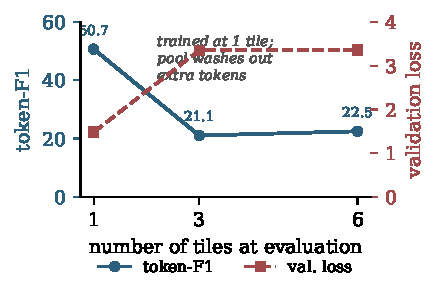
\includegraphics[width=0.62\linewidth]{fig_tile_collapse}
  \caption{\multitoken{} trained at one tile, evaluated at $\{1,3,6\}$ tiles:
  token-F1 (left axis) and validation loss (right axis).}
  \label{fig:tile-collapse}
\end{figure}

\subsection{Adaptive routing (RQ4) and training signal / alignment (RQ5)}
\label{sec:abl-routing}
\label{sec:abl-rq5}

\textbf{RQ4 --- can a policy spend the tile lever adaptively per question?} No.
An exhaustive oracle over the $(\text{bridge} \times \ntiles)$ action space
(Sec.~\ref{sec:method-adaptive}) beats the best fixed action
\bridge{multi\_token$|$t1} by $+0.36$ CIDEr on held-out test, spread \emph{evenly}
across all eight reasoning categories. But that headroom is not learnable: a
policy trained \emph{and} tested on the same split reproduces the oracle, yet
$a^\ast$ does not transfer (per-sample CIDEr on 4-word answers is a poor
estimator among near-tied actions). All three held-out policy arms
($P(r{\mid}Q)$, visual state $f(I,Q)$, or both) converge onto
\bridge{fixed: multi\_token$|$t1}, picking it for $\ge 97.9\%$ of test questions;
adding the reasoning-type posterior changes nothing.

\textbf{RQ5 --- does a better training target or vision--language alignment
help?} No (Table~\ref{tab:abl-summary}). Multi-reference answer sampling slightly
hurts (\dF{}~$-1.47$); distilling the bridge toward Vintern's \emph{own}
pre-aligned \texttt{mlp1} projector is an \textbf{absolute null}
(feature-KD \dF{}~$-0.03$) --- the bridge is already at the alignment the frozen
decoder can use. Logit-level KD confirms it: a null at $\alpha=0.1$
(\dF{}~$+0.20$, val CE $1.53$ vs.\ plain $1.49$) and destructive only at
$\alpha=1.0$ (\dF{}~$-8.80$, val CE $2.05$), where the KL term simply overwhelms
the CE loss --- not evidence that better-tuned alignment would help. Two KD
variants at two strengths: representation alignment does nothing for this frozen
decoder.

\subsection{Decoder capacity: LoRA (RQ6)}
\label{sec:abl-rq6}

\textbf{RQ6 --- does opening the decoder itself help?} \textbf{Yes --- this is the
one axis that moves F1}, and it is the only intervention that touches the
decoder.

\paragraph{Bridge-equalizing.}
Table~\ref{tab:abl-bridges} gives the LoRA lift for each bridge. The five plain
bridges span F1 $45.2$--$49.6$ / CIDEr-D $79$--$92$ --- real quality differences
across three token-mixing designs. After a $0.23\%$ LoRA on the decoder,
\textbf{all five converge to F1 $52.6$--$53.5$ / CIDEr-D $100.8$--$103.3$}
(Fig.~\ref{fig:bridge-equalizing}); the lift is larger for weaker bridges
($+4.0 \to +7.8$), and every plain$\to$LoRA CI clears zero. Once the decoder has
capacity to use whatever representation it is given, \emph{which bridge supplies
it stops mattering}.

\begin{figure}[t]
  \centering
  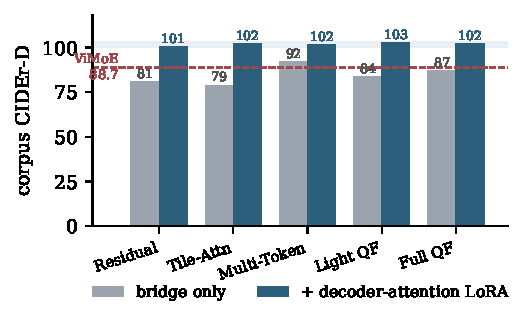
\includegraphics[width=0.68\linewidth]{fig_bridge_equalizing}
  \caption{Corpus CIDEr-D per bridge, bridge-only (grey) vs.\ + decoder-attention
  LoRA (colour). The $79$--$92$ spread collapses into a $101$--$103$ band.}
  \label{fig:bridge-equalizing}
\end{figure}

\paragraph{Where in the decoder.}
The usable headroom is \textbf{specifically in attention}. A same-rank LoRA on the
feed-forward blocks ($\text{gate}/\text{up}/\text{down}$) diverges training
(F1 $20.2 \pm 1.5$, val loss ${\sim}3.7$); on all seven modules it still diverges
(F1 $37.5 \pm 1.7$, val loss ${\sim}2.1$). \emph{Caveat:} this may be a
hyperparameter artefact ($\alpha=32$ is likely too strong for the wider MLP
dimension); we scope the claim to the recipe's configuration.

\paragraph{Rank and duration.}
A 3-seed rank sweep finds $r{=}16$, $32$ and $64$ statistically
indistinguishable (we keep $r{=}16$); training the LoRA for 3 epochs rather than 1
adds $+1.2$ F1 / $+4$ CIDEr-D and closes the gap to ViMoE to $6.0$, most of it by
epoch 2. The 1-epoch numbers are the headline, the 3-epoch the strongest form.

\subsection{Reading}
\label{sec:abl-summary}

Four independent axes on the vision / training side of the pipeline --- none of
which touch the decoder --- produce no lift; alignment KD is an
\emph{absolute} null across two variants and two strengths. The one axis that
touches the decoder produces a clear lift
on every bridge, and localizes further to the decoder's \textbf{attention}. This
\emph{pattern across six interventions} --- not any single ablation --- is what
localizes the bottleneck: for this VLM class (frozen ViT, frozen 0.5B decoder, a
few pooled vision tokens), the frozen decoder's attention is the ceiling, not the
vision pipeline. Opening it by $0.23\%$ recovers a third or more of the F1 gap to
a fully-unfrozen prior-work baseline. Sec.~\ref{sec:discussion} develops this
reading; the paper's primary contribution remains the ${\sim}1\%$ recipe of
Sec.~\ref{sec:results}.

\section{Human Validation and Error Analysis}
\label{sec:human}

Every result above is read through automatic metrics against five reference
answers. This section asks how much those metrics track answer \emph{correctness}.

\paragraph{Scope, stated up front.}
The planned protocol was 300--500 samples, 2 annotators, Cohen's $\kappa$; time
did not allow it before the deadline. What follows is a \textbf{single-rater
self-check substitute}, not human validation: $N = 120$, one rater, no image
access --- judged for plausibility against the five references only, a materially
weaker check for open-ended categories. Samples are drawn proportionally by
category $\times$ actual F1 bucket; all 120 judgments are released.

\begin{table}[t]
  \centering
  \caption{F1 bucket vs.\ semantic judgment (\multitoken{}, $N=120$).
  ``Acceptable'' $=$ correct $+$ partially correct ($\%$).}
  \label{tab:human}
  \begin{tabular}{lrrrrrr}
    \toprule
    F1 bucket & $n$ & correct & partial & wrong & nonsense & acceptable \\
    \midrule
    strong ($\ge 0.6$)    & 45 & 80.0 & 11.1 & 6.7  & 2.2 & \textbf{91.1} \\
    partial ($0.2$--$0.6$) & 58 & 12.1 & 31.0 & 55.2 & 1.7 & \textbf{43.1} \\
    weak ($0$--$0.2$)     & 3  & 0    & 0    & 100  & 0   & \textbf{0} \\
    zero ($\text{F1}=0$)  & 13 & 7.7  & 7.7  & 76.9 & 7.7 & \textbf{15.4} \\
    \midrule
    \textbf{total ($n=119$)} & & \textbf{37.0} & \textbf{20.2} & \textbf{40.3} & \textbf{2.5} & \textbf{57.1} \\
    \bottomrule
  \end{tabular}
\end{table}

The ``strong'' bucket ($\ge 0.6$ F1) is reliable ($91.1\%$ acceptable), but the
\textbf{``partial'' bucket ($0.2$--$0.6$) --- the \emph{largest} single bucket,
$51.5\%$ of val --- is only $43.1\%$ acceptable}, $55.2\%$ actually wrong despite
non-zero token overlap. The errors are not random noise (wrong colour / count /
object, or the wrong facet of the question), which is why they still score
mid-range F1. Overall $37.0\%$ of val predictions are fully correct, $57.1\%$
acceptable. \textbf{Mid-range token-F1 is not a reliable correctness signal},
which qualifies how the CIDEr-D / F1 numbers elsewhere should be read. A real
2-annotator, image-access study remains the camera-ready item.

\section{Discussion and Limitations}
\label{sec:discussion}

\subsection{Four vision/training axes, one language axis: localizing the ceiling}

Sec.~\ref{sec:abl-bridge}--\ref{sec:abl-rq6} push on four vision- and
training-side levers that could, in principle, close the remaining F1 gap to
ViMoE-VQA on top of the frozen-backbone, 1-tile bridge --- bridge capacity,
visual-compute allocation, training target and representation alignment --- plus
one language-side lever, decoder capacity. The four vision/training axes are
negative and only the decoder axis is positive --- and even there, only when the
LoRA is placed on the decoder's \emph{attention} projections. The shape of that
split is itself the finding:

\begin{enumerate}
\item \textbf{A bigger bridge does not help; the bridge is not the constraint
  (Sec.~\ref{sec:abl-bridge}).} A $10\times$-larger connector (the 69\,M-parameter
  Full Q-Former) is \emph{worse} than the 7\,M-parameter multi-token bridge on
  both F1 ($-2.2$) and CIDEr-D, and the multi-token bridge already has the lowest
  validation cross-entropy of all five architectures. Whatever the decoder cannot
  do with eight pooled tokens, it also cannot do with sixteen learned queries and
  four fusion layers.
\item \textbf{Reasoning type does not predict visual-compute demand
  (Sec.~\ref{sec:abl-routing}).} Per category, the effect of \ntiles{} on answer
  quality is not significant in any of the eight categories; no learned policy ---
  reasoning-type-informed or not --- beats a fixed \bridge{multi\_token$|$t1} on
  held-out test. This holds on both the original and the tile-count-augmented
  retrained checkpoints, so it is not an artefact of the bridge never having seen
  $>1$ tile during training.
\item \textbf{Multi-reference training and projector-alignment KD do not lift F1
  (Sec.~\ref{sec:abl-rq5}).} Neither training on a resampled reference each epoch
  (\dF{}~$-1.5$) nor distilling the bridge toward Vintern's own pre-aligned
  \texttt{mlp1} projector (\dF{}~$-0.03$, an \emph{absolute} null) moves F1
  upward. The bridge is already close to CE-optimal
  (Sec.~\ref{sec:abl-bridge}) --- there is little room for a training-signal or
  alignment tweak to improve on.
\item \textbf{Decoder-LoRA is the one intervention that moves F1, it is
  bridge-agnostic, and it works only on the attention projections
  (Sec.~\ref{sec:abl-rq6}).} Adapting $0.23\%$ of Qwen2-0.5B's parameters lifts
  F1 $+3.6$ on \multitoken{} and $+5.9$--$7.8$ on the four other bridges --- a
  \emph{larger} effect on the weaker bridges, which rules out ``one bridge's LoRA
  got lucky''. After LoRA all five bridges collapse into a $0.6$-point F1 band and
  a $2.6$-point CIDEr-D band, from plain spreads of ${\sim}4.4$ F1 / ${\sim}13$
  CIDEr-D. Moving the same LoRA budget to the decoder's feed-forward layers
  \emph{diverges} training (val loss $2$--$4$ vs.\ $1.37$, F1 $20$--$38$); the
  useful headroom is specifically in attention, not the decoder broadly. (We flag
  the MLP result as possibly a hyperparameter artefact --- $\alpha=32$ is
  aggressive for the larger intermediate dimension --- so the claim is scoped to
  the recipe's settings.)
\end{enumerate}

\paragraph{Reading.}
Every vision- and training-side lever produces no lift (alignment is a flat
zero); the one lever that touches the decoder produces a lift on every bridge,
and only through its attention projections. That pattern is more informative than
any single ablation: it is not that we tried one clever trick and it happened to
work, it is that \emph{only} the trick which adds attention capacity to the
decoder worked, regardless of which bridge. For this VLM class --- frozen ViT,
frozen small (0.5B) decoder, a few pooled vision tokens --- the frozen decoder is
the ceiling on token-level phrasing match, not the vision pipeline. We report
LoRA as a reference point quantifying that ceiling, not as a replacement for the
paper's main spine (Sec.~\ref{sec:results-main}--\ref{sec:results-corpus}) --- the
frozen, $0.78\%$-param bridge remains the primary contribution, and this finding
explains why that architecture class tops out where it does rather than arguing
it should be abandoned.

\subsection{Relation to ViMoE-VQA's ``reasoning-aware'' claim}

ViMoE-VQA attributes part of its MoE gain to ``approximate reasoning-aware expert
selection''. Our result does not contradict ViMoE's accuracy numbers, but it does
suggest the mechanism is mis-attributed: on the same benchmark, reasoning type
carries no signal about the \emph{optimal} visual-compute action, and ViMoE's own
leave-one-out ablation shows its experts are not strongly specialised. A more
parsimonious account of the MoE gain is added capacity / ensembling, not
reasoning-type routing. Testing this on ViMoE directly (does expert activation
correlate with question type?) is the obvious follow-up and requires only its
router logs.

\subsection{What is robust}

\begin{itemize}
\item The \textbf{grouped split} closes an image-level leakage path; our bridge
  numbers are essentially unchanged from the random-split table
  ($\le 0.5$ F1 / $\le 3$ CIDEr-D). \emph{Caveat:} one early Residual-bridge run
  used in the first comparison was a training-instability outlier (val CE $2.35$
  vs.\ ${\sim}1.5$--$1.7$ elsewhere); with a sound 3-seed run the Residual numbers
  rise sharply (F1 $36.5{\to}45.6$, CIDEr-D $56.3{\to}81.1$) --- so the ``barely
  changed'' claim holds for the four stable bridges, not for that single broken
  run.
\item The \textbf{multi-token bridge} result --- corpus CIDEr-D $92.3$ / BLEU-4
  $18.9$ / ROUGE-L $48.9$ on val, above ViMoE-VQA on all three, at $0.78\%$
  trainable parameters --- holds across 4 seeds and \textbf{on held-out test}
  (F1 $49.2$ vs.\ val $49.6$), a clean, reproducible positive with no val-set
  overfitting.
\item The \textbf{compute-efficiency characterisation}
  (Sec.~\ref{sec:abl-compute}) is the FLOPs/latency analysis ViMoE-VQA explicitly
  deferred.
\item The \textbf{null result on adaptive visual-compute routing}
  (Sec.~\ref{sec:abl-routing}) is cross-validated on two independently-trained
  checkpoint generations --- the same conclusion both times rules out ``the
  bridge just never learned to use tiles'' as a confound.
\item The \textbf{decoder-LoRA result} (Sec.~\ref{sec:abl-rq6}) is the
  most-replicated finding in the paper: $+3.6$ F1 on \multitoken{} (3/3 seeds) and
  $+5.9$--$7.8$ on four other bridges, all converging to a $0.6$-point F1 band;
  confirmed at corpus level and on held-out test. Three checks (seed, bridge,
  metric implementation) plus the attention-vs-MLP contrast all agree.
\end{itemize}

\subsection{Limitations}

\begin{enumerate}
\item \textbf{3-seed, not 5.} Bridge and negative-axis runs are 3 seeds
  (\multitoken{} 4); routing/oracle runs are seed 42. A 5-seed protocol is the
  camera-ready target.
\item \textbf{Frozen 0.5\,B decoder.} The negative routing/training/alignment
  results may not generalise to VLMs with a trainable or larger decoder that
  \emph{can} use extra visual tokens --- and Sec.~\ref{sec:abl-rq6}'s LoRA result
  is direct evidence for exactly that. We claim the negatives for the
  frozen-backbone / small-bridge regime only.
\item \textbf{Decoder-LoRA epoch and rank grid is coarse.} The MLP / attn+MLP
  divergence uses the recipe's $\alpha=32$ and learning rate --- a lower $\alpha$
  or longer schedule might make MLP LoRA viable. Treat the \emph{direction and
  bridge-agnosticism} of the effect as solid, the exact magnitude as provisional.
\item \textbf{$\ntiles \in \{1,3,6\}$ and three oracle bridges.} A finer action
  grid, or bridges that consume per-tile tokens without pooling, might expose
  structure this study cannot see.
\item \textbf{$M(a;x) =$ per-sample CIDEr} is noisy for 4-word answers; a less
  noisy per-sample quality signal (\eg an LLM judge) could in principle recover
  some headroom.
\item \textbf{Cross-paper metric implementations.} Baseline rows are as-reported
  and may use different implementations, especially for METEOR and BLEU; we
  standardise our own numbers on pycocoevalcap.
\item \textbf{Oracle-sweep subset} is equal-per-category; overall numbers are
  re-weighted but tail categories are over-represented in the raw sweep.
\item \textbf{Human validation is done only in reduced form.}
  Sec.~\ref{sec:human} substitutes a single-rater self-check ($N=120$, no image
  access) for the planned 2-annotator, Cohen's-$\kappa$ study; its finding is
  informative but rests on one rater's judgment without an image.
\end{enumerate}

\subsection{Ethical and reproducibility notes}

All models are frozen public checkpoints; only small bridges/heads are trained.
The split script, action space, and oracle tables are released. No human-subjects
data beyond the public AutoViVQA benchmark.

\section{Conclusion}
\label{sec:conclusion}

We asked whether Vintern-1B can be improved on AutoViVQA by training only a small
fraction of its parameters, and where the bottleneck lies. A frozen InternViT-300M
and frozen Qwen2-0.5B, connected by a $0.78\%$ mean-pooled bridge at one tile and
adapted with a $0.23\%$ rank-16 attention LoRA on the decoder, matches or beats
the fully fine-tuned Vintern-1B on every generation metric and beats ViMoE-VQA on
corpus CIDEr-D / BLEU-4 / ROUGE-L --- at ${\sim}1\%$ trainable parameters, one
16\,GB GPU, no backbone fine-tuning, and with held-out test numbers matching
validation.

Across a six-question ablation ladder, four vision- and training-side levers ---
a $10\times$-larger bridge, more tiles, a per-question routing policy,
multi-reference training, projector-level alignment --- produce no F1 improvement
(alignment is an exact null). The only lever that helps is a small LoRA on the
frozen decoder; it helps on every bridge, works only through the attention
projections (feed-forward LoRA destabilises training), and collapses the five
bridges into a $0.6$-point F1 band. For this VLM class, the ceiling on
token-level phrasing is the frozen decoder's attention capacity, not the visual
pipeline --- and on the same benchmark, question type carries no signal about the
optimal visual-compute action, a direct counterpoint to ``reasoning-aware''
routing accounts.

We release the code, the leak-free grouped split, the per-question oracle tables,
and all checkpoints. The natural next step is to vary the one component we kept
frozen and small --- the decoder --- and test whether a larger frozen Vietnamese
decoder closes the remaining token-F1 gap without any of the levers that failed
here.


\bibliographystyle{splncs04}
\bibliography{references}

\end{document}
